\section{Auswertung}
\label{sec:Auswertung}

%Bragg
\subsection{Überprüfung der Bragg-Bedingung}
Die gemessenen Daten (Tab. \ref{tab:bragg}) sind in der Abb. \ref{fig:bragg2} graphisch dargestellt.
\begin{figure}
    \centering
    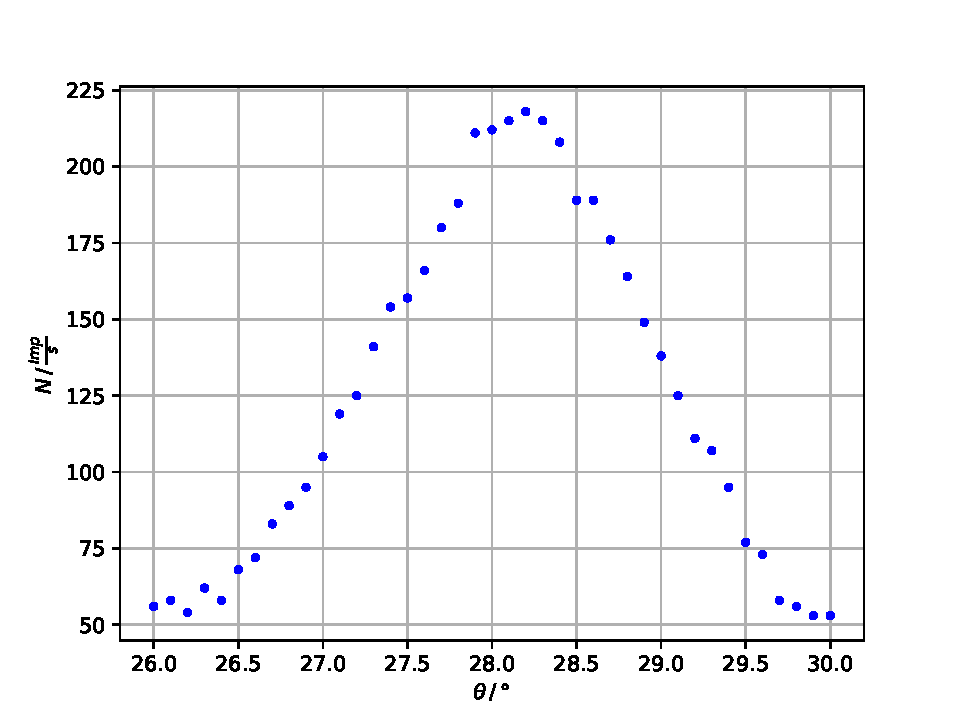
\includegraphics[width=0.8\textwidth]{content/data/bragg.pdf}
    \caption{Gemessener Impuls $N$ bei bestimmten Winkel $\theta$ zur Überprüfung der Bragg-Bedingung. \cite{numpy} \cite{matplotlib}}
    \label{fig:bragg2}
\end{figure}
Das experimentelle Maximum befindet sich bei
\begin{equation*}
    \theta_\text{exp} = \SI{28.2}{\degree} .
\end{equation*}
Nach der theoretischen Erwartung (Reflexionsgesetz), liegt das Maximum bei
\begin{equation*}
    \theta_\text{th} = \SI{28.0}{\degree}
\end{equation*}
für den Einfallswinkel $\theta_\text{ein}=\SI{14}{\degree}$ .

%Emissionsspektrum
\subsection{Analyse eines Emissionsspektrums der Kupfer-Röntgenröhre}
Die Messdaten zum Emissionsspektrum der Kupfer-Röntgenröhre befinden sich in Tab. \ref{tab:spektrum1}.
In Abb. \ref{fig:emission} sind die Daten graphisch dargestellt.
\begin{figure}
    \centering
    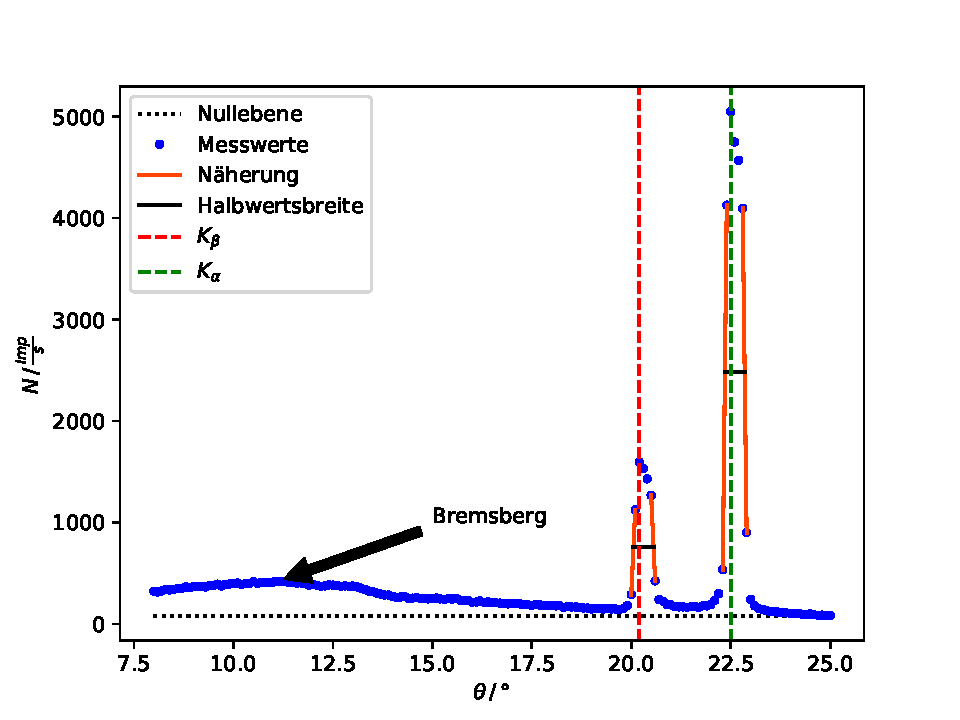
\includegraphics[width=0.8\textwidth]{content/data/plot.pdf}
    \caption{Messdaten, charakteristische Linien und Halbwertsbreiten zum Emissionsspektrum der Kupfer-Röntgenröhre. \cite{numpy} \cite{matplotlib} \cite{scipy}}
    \label{fig:emission}
\end{figure}
Die Nulllinie wird auf den niedrigsten Messwert gesetzt.
Im letzten Versuch V603 wurde bereits gezeigt, dass der erste Peak der $K_\beta$-Linie und der zweite Peak der $K_\alpha$-Linie entspricht.
Die charakteristischen Linien befinden sich bei
\begin{align*}
    \theta_{K,\beta} = \SI{20.2}{\degree} \\
    \theta_{K,\alpha} = \SI{22.5}{\degree} .
\end{align*}
Die maximale Energie an den charakteristischen Linien, ergibt sich aus der Bragg-Bedingung \eqref{eqn:lambdaalpha} und der Energie $E = \frac{hc}{\lambda}$:
\begin{align*}
    E_{K,\beta} = \SI{1.43e-15}{\joule} \\
    E_{K,\alpha} = \SI{1.29e-15}{\joule}
\end{align*}
Um den $K_\alpha$, $K_\beta$-Linien befinden sich wenige Messwerte, so dass nicht direkt die Halbwertsbreite bestimmt werden kann.
Zur Annäherung werden Geraden verwendet, welche die nächsten beiden Messwerte zur Halbwertsbreite verbinden.
Die Halbwertsbreite beschreibt hier die Energiedifferenz bei der hälfte der charakteristischen Linien:
\begin{align*}
    \Delta E_{\beta, FWHM} = \SI{3.38e-17}{\joule} \\
    \Delta E_{\alpha, FWHM} = \SI{2.67e-17}{\joule}
\end{align*}
Nach \eqref{eqn:aufloesung} wird das Auflösungsvermögen beider Linien bestimmt:
\begin{align}
    A_\beta = 42.23 \\
    A_\alpha = 48.27
    \label{eqn:erg_A}
\end{align}
Mithilfe der Absorptionsenergie $E_\text{abs} = \SI{8.9789}{\kilo\electronvolt}$ \cite{k_kante}, der Ordnungszahl für Kupfer $z = 29$ und der Rydbergenergie $R_\infty = \SI{13.6}{\electronvolt}$, können die Abschirmkonstanten \eqref{eqn:sigma1}, \eqref{eqn:sigma2}, \eqref{eqn:sigma3} bestimmt werden:
\begin{align}
    \sigma_1 = 3.31 \\
    \sigma_2 = 12.41 \\
    \sigma_3 = 22.45
    \label{eqn:erg_abschirm}
\end{align}

%Absorption
\subsection{Analyse der Absorptionsspektren}
Zum Schluss werden die Absorptionsspektren von 6 Elementen untersucht.
Zuerst sind die Theoriewerte \cite{k_kante} in Tab. \ref{tab:theorie} aufgeführt.
\begin{table}
    \centering
    \begin{tabular}{c|cccc}
    \toprule
    Element & Z & $E_{K, th} \,/\, \si{\femto\joule}$ & $\theta_{K, th} \,/\, \si{\degree}$ & $\sigma_{K, th}$ \\
    \midrule
    Zink & 30 & 1.55 & 18.56 & 3.55 \\
    Gallium & 31 & 1.66 & 17.27 & 3.61 \\
    Brom & 35 & 2.16 & 13.21 & 3.84 \\
    Rubidium & 37 & 2.44 & 11.68 & 3.94 \\
    Strontium & 38 & 2.58 & 11.02 & 3.99 \\
    Zirkonium & 40 & 2.88 & 9.85 & 4.09 \\
    \bottomrule
    \end{tabular}
    \caption{Theoriewerte der Absorptionsenergie, des Braggwinkels und der Abschirmkonstante $\sigma_K$. \cite{k_kante}}
    \label{tab:theorie}
\end{table}
\FloatBarrier

Die experimentell gemessenen Daten befinden sich in Tab. \ref{tab:znba}, \ref{tab:brrb} und \ref{tab:srzr}.
Die Intensität in der Mitte der Kante $I_K$
\begin{equation*}
    I_K = I_{K,min} + \frac{I_{K,max} - I_{K,min}}{2}
\end{equation*}
berechnet sich aus den maximalen $I_{K,max}$ und minimalen $I_{K,min}$ Intensitäten.
Liegt der errechnete Wert zwischen zwei Messwerten, so wird der nähere Messwert verwendet.
\\
Aus der Intensität $I_K$ wird die Absorptionsenergie $E_{K,abs}$ mithilfe der Bragg-Bedingung \eqref{eqn:lambdaalpha} bestimmt.
Die Abschirmkonstanten \eqref{eqn:abschirm_k} ergeben sich aus der Ordnungszahl $Z$ des jeweiligen Elements und der Konstanten $R_\infty$ \cite{anleitung}, $\alpha = \SI{7.29735e-3}{}$ \cite{konst}.
\\
Die berrechneten Daten befinden sich für die jeweiligen Elemente in Tab. \ref{tab:erg_elemente}.
In den Abb. \ref{fig:elemente} sind die Daten graphisch dargestellt.
Konstanten wie $R_\infty$, $\alpha$, $c$ \cite{konst} und $d$ \cite[3]{anleitung} werden der Literatur entnommen.
\begin{table}
    \centering
    \begin{tabular}{c|ccccccc}
    \toprule
    Element & $I_{K,max} \,/\, \si{\frac{Imp}{s}}$ & $I_{K,min} \,/\, \si{\frac{Imp}{s}}$ & $I_{K} \,/\, \si{\frac{Imp}{s}}$ & $\theta_K \,/\, \si{\degree}$ & $E_{K} \,/\, \si{\femto\joule}$ & $\sigma_K$ & Abb. \\
    \midrule
    Zink & 102.0 & 54.0 & 78.0 & 18.7 & 1.54 & 3.63 & \ref{fig:zink} \\
    Gallium & 122.0 & 66.0 & 94.0 & 17.3 & 1.66 & 3.64 & \ref{fig:gallium} \\
    Brom & 27.0 & 9.0 & 18.0 & 13.2 & 2.16 & 3.84 & \ref{fig:brom} \\
    Rubidium & 64.0 & 10.0 & 37.0 & 11.8 & 2.41 & 4.11 & \ref{fig:rubidium} \\
    Strontium & 196.0 & 40.0 & 118.0 & 11.1 & 2.56 & 4.12 & \ref{fig:strontium} \\
    Zirkonium & 301.0 & 112.0 & 206.5 & 10.0 & 2.84 & 4.37 & \ref{fig:zirkonium} \\
    \bottomrule
    \end{tabular}
    \caption{Minimale $I_{K,min}$, maximale $I_{K,max}$ und mittlere Intensität $I_K$ beim Winkel $\theta_K$ für jedes Element aufgelistet. Aus dem Winkel resultiert die Absorptionsenergie $E_K$ und die Abschirmkonstante $\sigma_K$.}
    \label{tab:erg_elemente}
\end{table}

% 6 graphiken der elemente
\begin{figure}[t!] % "[t!]" placement specifier just for this example
\begin{subfigure}{0.48\textwidth}
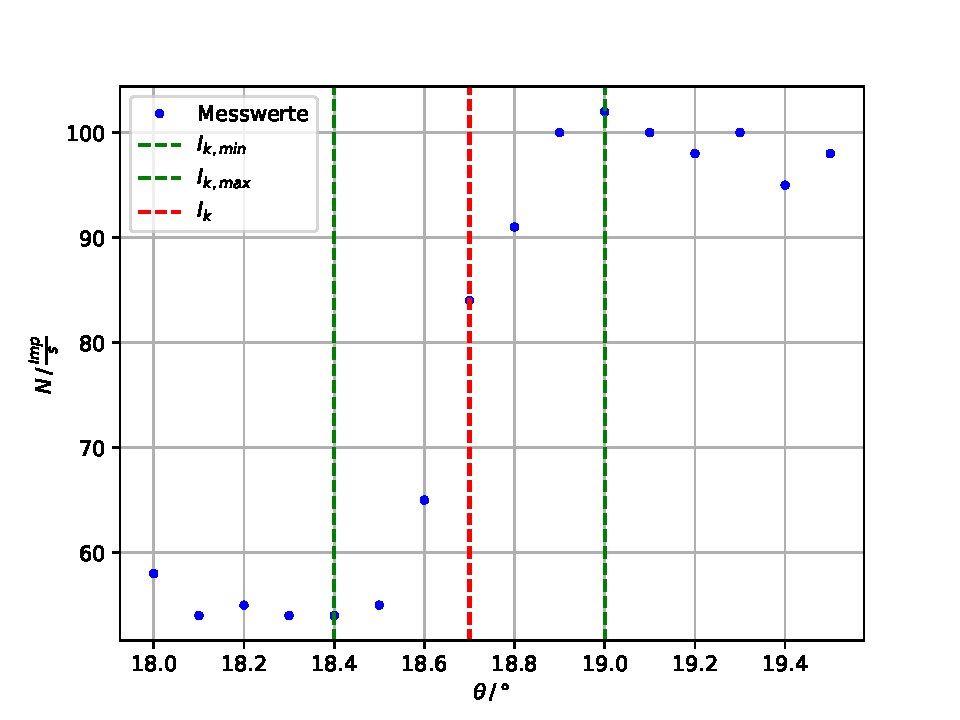
\includegraphics[width=\linewidth]{content/data/zink.pdf}
\caption{Zink} \label{fig:zink}
\end{subfigure}\hspace*{\fill}
\begin{subfigure}{0.48\textwidth}
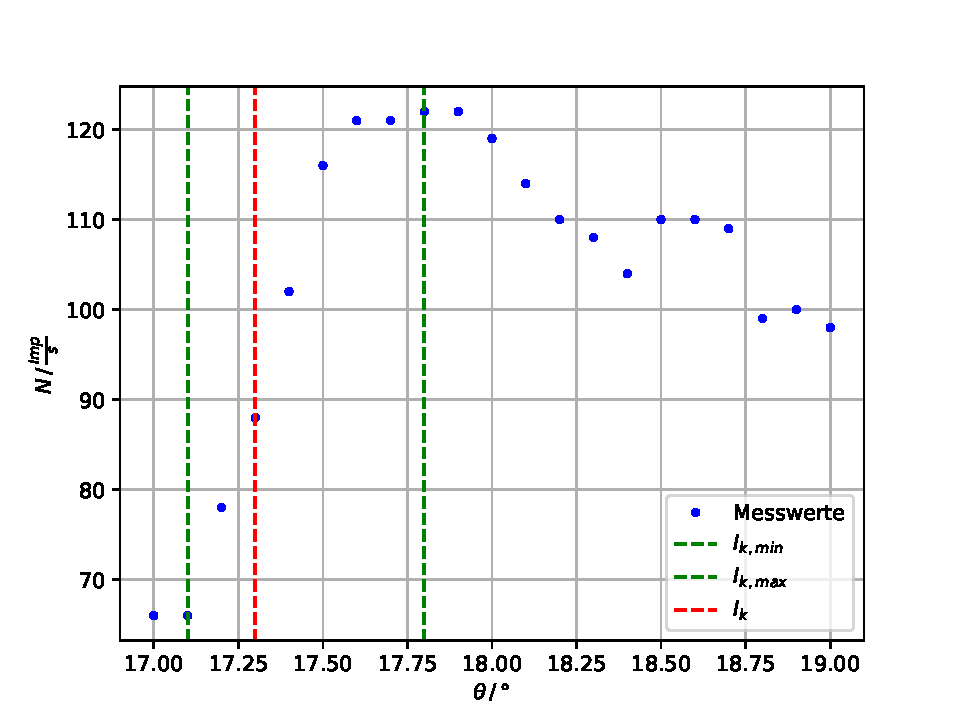
\includegraphics[width=\linewidth]{content/data/gallium.pdf}
\caption{Gallium} \label{fig:gallium}
\end{subfigure}

\medskip
\begin{subfigure}{0.48\textwidth}
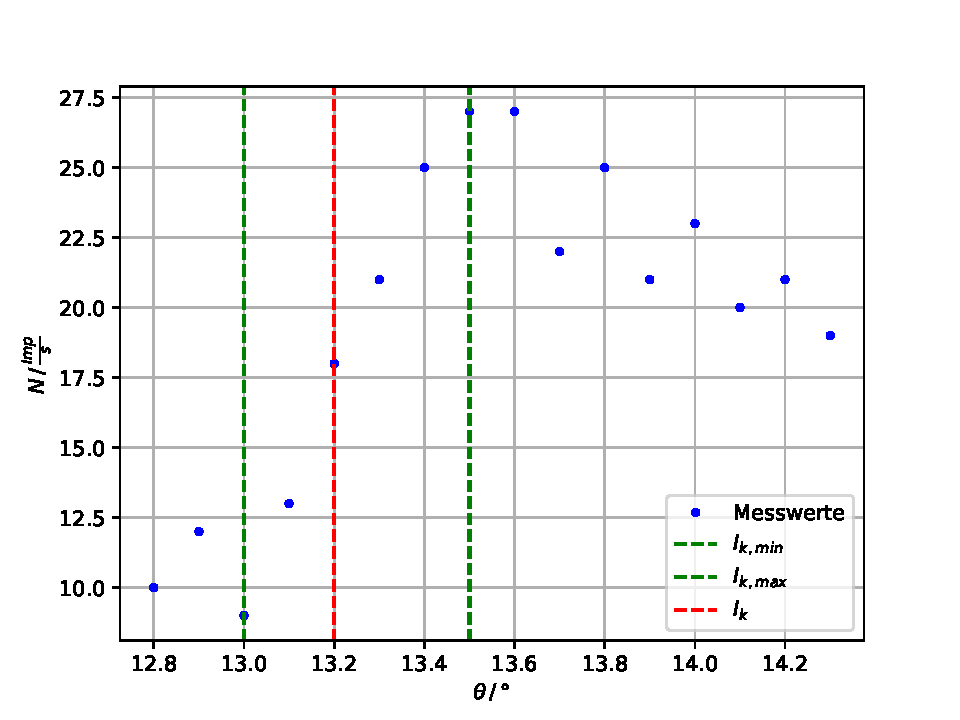
\includegraphics[width=\linewidth]{content/data/brom.pdf}
\caption{Brom} \label{fig:brom}
\end{subfigure}\hspace*{\fill}
\begin{subfigure}{0.48\textwidth}
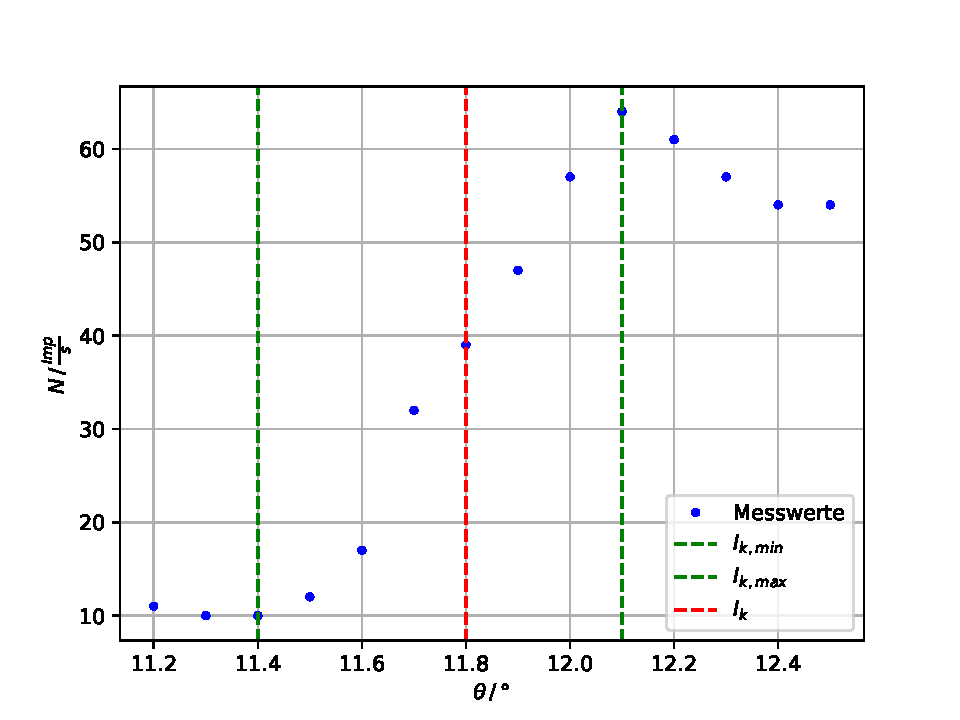
\includegraphics[width=\linewidth]{content/data/rubidium.pdf}
\caption{Rubidium} \label{fig:rubidium}
\end{subfigure}

\medskip
\begin{subfigure}{0.48\textwidth}
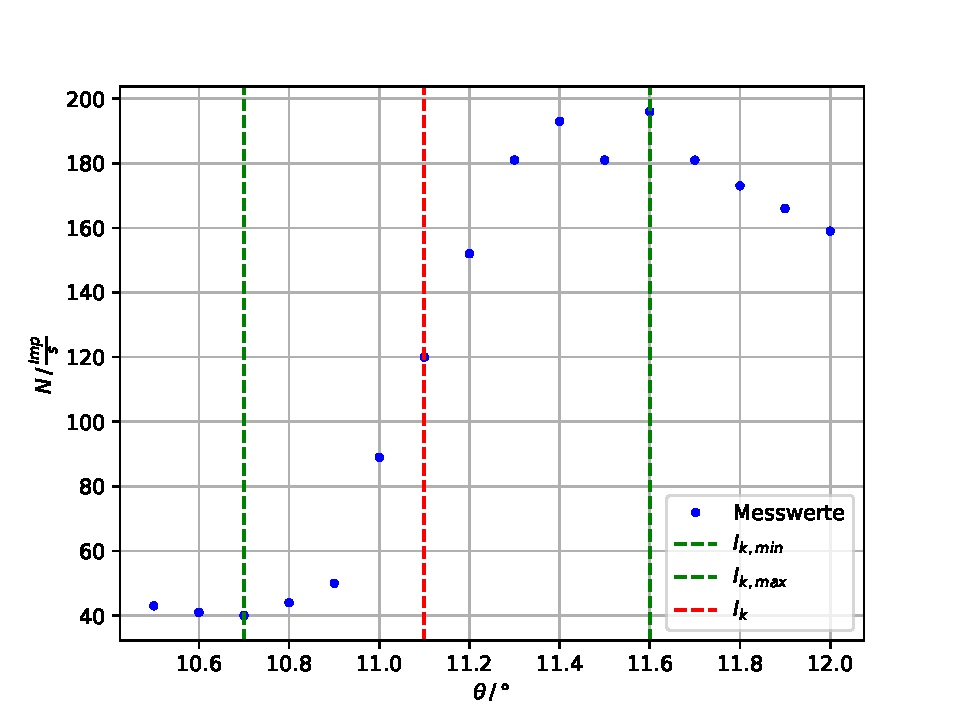
\includegraphics[width=\linewidth]{content/data/strontium.pdf}
\caption{Strontium} \label{fig:strontium}
\end{subfigure}\hspace*{\fill}
\begin{subfigure}{0.48\textwidth}
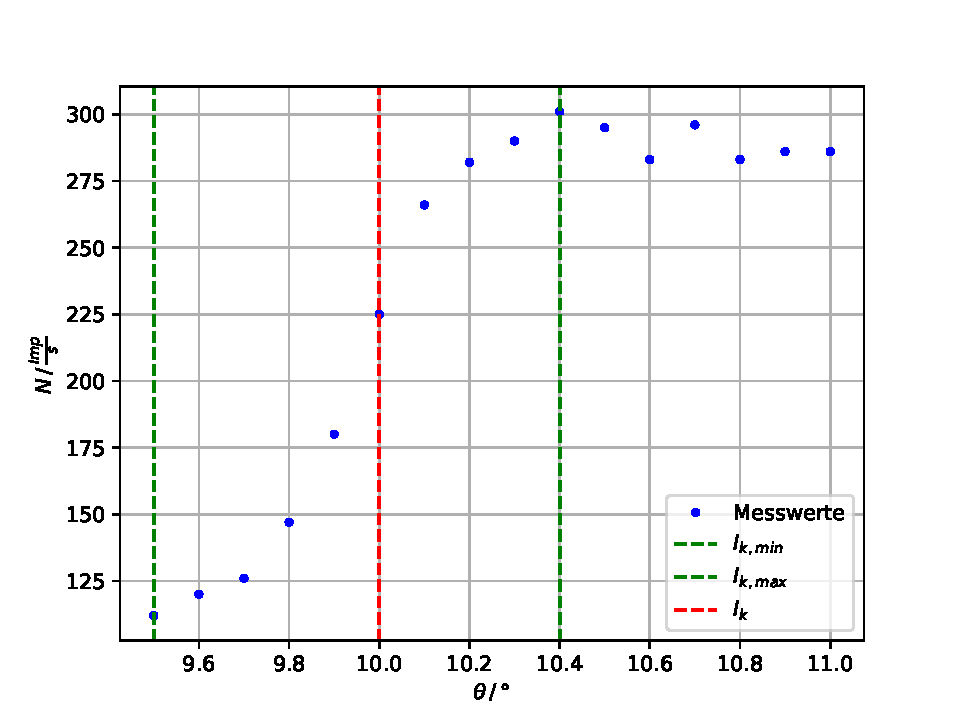
\includegraphics[width=\linewidth]{content/data/zirkonium.pdf}
\caption{Zirkonium} \label{fig:zirkonium}
\end{subfigure}
\caption{Messdaten, Intensitätsminimum, -maximum und -mitte des Absorptionsspektrum des jeweiligen Elements graphisch dargestellt. \cite{numpy} \cite{matplotlib}}
\label{fig:elemente}
\end{figure}

\FloatBarrier

Aus dem Moseley'schen Gesetz \eqref{eqn:moseley} und einer linearen Ausgleichsrechnung
\begin{equation*}
    \sqrt{E_K} = a \cdot z + b
\end{equation*}
mit den Parametern
\begin{align*}
    a = \sqrt{R \cdot h} \\
    b = -\sqrt{ R\cdot h} \cdot \sigma
\end{align*}
ergibt sich die Rydbergfrequenz
\begin{equation*}
    R_\text{exp} = \SI{2.99(5)e15}{\hertz} .
\end{equation*}
Daraus folgt für die Rydbergenergie
\begin{equation}
    R_{\infty ,exp} = h \cdot R = \SI{1.981(30)e-18}{\joule} .
\end{equation}
Die Ausgleichsgerade und die verwendeten Messwerte sind in Abb. \ref{fig:ausgleich} graphisch dargestellt.
\begin{figure}
    \centering
    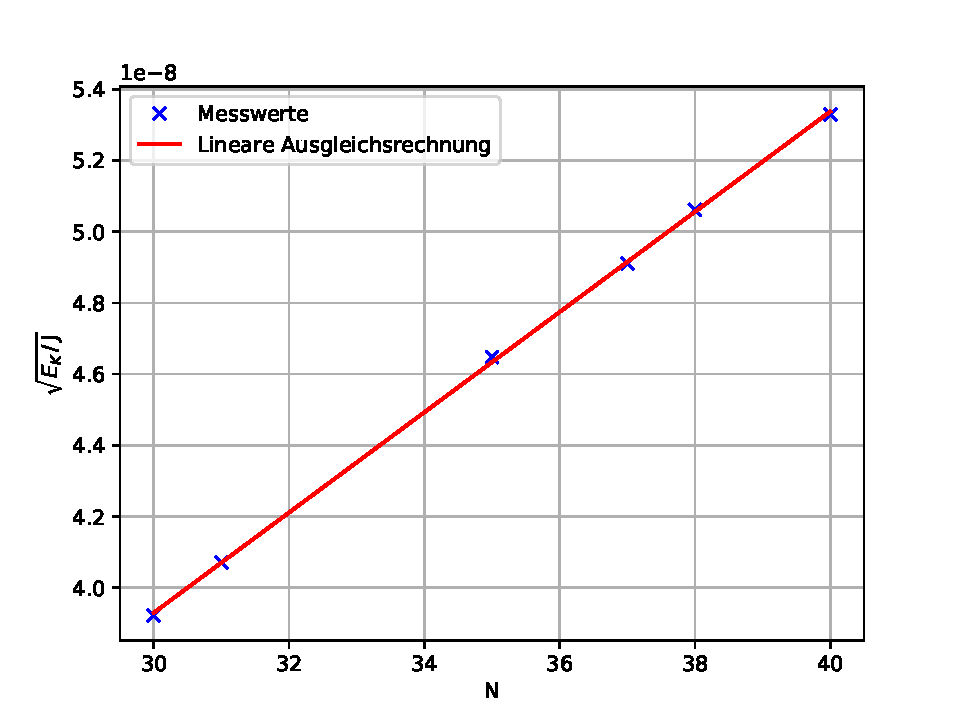
\includegraphics[width=0.8\textwidth]{content/data/ausgleich.pdf}
    \caption{Lineare Ausgleichsrechnung zur Bestimmung der Rydbergfrequenz. \cite{numpy} \cite{matplotlib} \cite{scipy}} 
    \label{fig:ausgleich}
\end{figure}
\FloatBarrier
Der theoretische Wert der Rydbergenergie \cite{konst}
\begin{equation*}
    R_{\infty ,th} = \SI{2.179871e-18}{\joule}
\end{equation*}
wird der Literatur entnommen.